\chapter{Examples}
\label{chap:examples}
In this section, we provide some examples to show the main capabilities of \mpng{} for simulating the operation of power and natural gas networks. We have included the folder \mpngcasepath{} in the distribution, which contains the gas and interconnection cases used for testing. Moreover, the folder \mpngexamplepath{} contains the files used in the examples. In particular, we explore two examples: (1) the integrated operation of a nine-bus power system  and an eight-node natural gas grid; and (2) the single operation of a 48-node looped natural gas network.

\section{9-bus 8-node Power\&Gas System}
\label{sec:8-9_gas_power}

We analyze an interconnected system formed by a power system of nine buses  and a natural gas network of eight nodes. As shown in Figure \ref{fig:example1}, they are coupled through a gas-fired power plant and a power-driven compressor working with energy coming from the power system. This example aims aimed at showing the primary functionalities of \mpng{} as well as how to properly run a simulation. 

The power system consists of the classic \matpower{} nine-bus case, with some modifications in order to meet the requirements of the interconnected network. Some of these changes are related to bus areas, line capability constraints, maximum power generation, and generation costs. For the gas system, we created an eight-node looped case with two compressors connected in series and a loop formed by three pipelines. Tables \ref{tab:ex1_power} and \ref{tab:ex1_gas} summarize the system information. 

\begin{figure}[!ht]
	\centering
	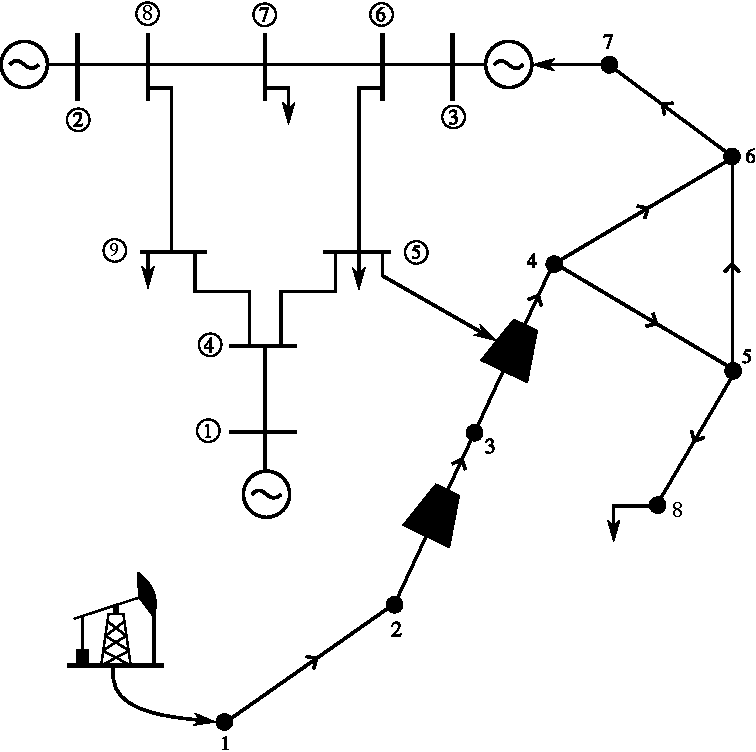
\includegraphics[scale=0.8]{Figures/Example1}
	\caption{Power and gas integrated network considered in Example 1.}
	\label{fig:example1}
\end{figure}


\begin{table}[!ht]
\centering
\begin{threeparttable}
\caption{Example 1 - Power System Summary}
\label{tab:ex1_power}
\footnotesize
\begin{tabular}{ll}
\toprule
\bf{topology}	& 9-bus network	 \\
\midrule
			& 3 gens at buses 1, 2, and 3\\
\bf{generators}	& 200 MW Max $P_{g}$ for all generators\\
			& all 3 have identical quadratic generation costs \tnote{*}\\
\midrule
\bf{load}		& 90 MW at bus 5, 100 MW at bus 7, 125 MW at bus 9 \\
			& curtailable at \$5000/MWh	\\
\midrule
\bf{branches}	& 250 MW limit for all lines	\\
\bottomrule
\end{tabular}
\begin{tablenotes}
 \scriptsize
 \item [*] {Linear costs of \$95/WMh are used for the example.}
\end{tablenotes}
\end{threeparttable}
\end{table}


\begin{table}[!ht]
%\renewcommand{\arraystretch}{1.2}
\centering
\begin{threeparttable}
\caption{Example 1 - Gas System Summary}
\label{tab:ex1_gas}
\footnotesize
\begin{tabular}{ll}
\toprule
\bf{topology}	& 8-node looped network	 \\
\midrule
			& 1 well at node 1\\
\bf{well}		& 80 MMSCF Max $g^{w}$ for well\\
			& linear cost extraction cost (\$5000 / MMSCFD )\\
\midrule
			& gas demands at nodes 7 and 8\\
\bf{load}		& 2 types of gas load 	\\
			& high cost of non-supplied demand\\
\midrule
\bf{pipelines}	& no active limits for all lines	\\
			& transport cost at (\$5 / MMSCFD) for all pipelines \\
\midrule
\bf{compressors}	& no active limits for all compressors	\\
			& transport cost at (\$5 / MMSCFD) for all compressors \\
\midrule
\bf{storage}	& no storage considered	\\			
\bottomrule
\end{tabular}
\begin{tablenotes}
 \scriptsize
 \item [] {}
\end{tablenotes}
\end{threeparttable}
\end{table}

Initially, for the sake of convenience and code portability, we define the column pointers (constants) for the power system\footnote{The default \matpower{} function \code{define\_constants} allows an straightforward indexing of all information via integer variables. See \cite{matpower_manual} for details.}. Similarly, we define column pointers to easily access the natural gas and interconnection cases, as follows:

\begin{Code}
>> define_constants        % power system constants
>> define_constants_gas    % natural gas system and connect struct constants
\end{Code}

We can load the \matpower{} options struct to chose the desired solver and some additional features. The current stable solver for \mpng{}  is `IPOPT'. Besides, based on the experience, we set the maximum number of iterations to 100000, as shown below:

\begin{Code}
>> mpopt = mpoption;                   % initialize option struct
>> mpopt.opf.ac.solver = `IPOPT';      % current stable solver
>> mpopt.ipopt.opts.max_iter = 1e5;    % max iterations
\end{Code}

Afterwards, we load the power and gas cases and the connection struct\footnote{All cases and connection struct are included in the folder \mpngcasepath{}. Since the data of the interconnection case mainly comprises additional information of the \matpower{}-case, we refer to the connect struct using a similar name as that used for the power system case.}. For the sake of simplicity, we name the power case as \code{mpc}, the natural gas case as \code{mgc},  and the connection struct as \code{connect}, as follows: 

\begin{Code}
>> mpc = loadcase(`case9_new');    % 9 bus power system
>> mgc = ng_case8;                 % 8 node natural gas system
>> connect = connect_pg_case9;     % interconnection case
\end{Code}

As the window of analysis consist in an entire day for the gas network, we just need to define the number of periods and their corresponding length for analyzing the power system. We consider four periods of time, each of them of the same length, that is:

\begin{Code}
>> connect.power.time = [6 6 6 6];   % four periods of time
\end{Code}

The connection struct also requires the active and reactive demands in all buses for each period. Then, we take the original system's demand to produce such a temporal behavior via a factor vector as follows:  

\begin{Code}
>> factors = [1 1.1 1.2 0.9];      % factors (external aid of MPNG)
>> connect.power.demands.pd = factors.*mpc.bus(:,PD);  % PD matrix
>> connect.power.demands.qd = factors.*mpc.bus(:,QD);  % QD matrix
\end{Code}

Moreover, we set the generator number two to have a maximum daily energy of 5000 MWh/d:

\begin{Code}
>> connect.power.energy = zeros(1,2);  % initialize (one gen with max energy)
>> connect.power.energy(1,GEN_ID) = 2;         % id for max energy in gen 2 
>> connect.power.energy(1,MAX_ENER) = 5000;    % max energy is 1000 MWh/d 
\end{Code}

For this particular example, we do not consider spinning reserve because of the small number of generators. As a consequence, the spinning reserve matrix is set to be an empty array:

\begin{Code}
>> connect.power.sr = [];                      % no spinning reserves
\end{Code}

As shown in Figure \ref{fig:example1}, both classes of compressors where included in this example. Their corresponding information, specified in the connection struct, must be consistent with the gas and power cases:

\begin{Code}
>> connect.interc.comp = zeros(1,2); % initialize (a power-driven compressor)
>> connect.interc.comp(1,COMP_ID) = 2;       % second compressor
>> connect.interc.comp(1,BUS_ID) = 5;        % connected to bus # 5
>> mgc.comp(2,TYPE_C) = COMP_P;              % concordance with gas case
\end{Code}

Additionally, a gas-fired power plant was considered, and its information must be included in the connection struct in a manner consistent with the gas and power cases:

\begin{Code}
>> connect.interc.term = zeros(1,3);       % initialize (one gas-fired plant)
>> connect.interc.term(1,GEN_ID)  = 3;     % third power plant
>> connect.interc.term(1,NODE_ID) = 7;     % connected to node # 7
>> connect.interc.term(1,EFF) = 10e-3;     % power plant eff. (MMSCFD/MWh)
\end{Code}

At this point, we have set all the inputs required to model the different aspects that we intended for the interconnected power and natural gas system. Now, we need to put all together in a single struct. We call this struct \code{mpgc}, which represents the combination between \code{mpc}, \code{mgc}, and \code{connect}, as shown below:

\begin{Code}
>> mpgc = mpc;                         % initialize MPNG case
>> mpgc.mgc = mgc;                     % adding gas case
>> mpgc.connect = connect;             % adding connection struct
\end{Code}

Finally, we can run the simulation by calling \mpng{} using the \code{mpgc} case and the \matpower{} options struct:
 
\begin{Code}
>> results = mpng(mpgc,mpopt);         % running simulation
\end{Code}

The optimal solution values are saved as the \code{results} struct.  See Section \ref{subsec:view_results} for more details about the simulation \code{results}. By default, the \code{results} are pretty-printed. The information related to the natural gas network after running the simulation looks like:\\

\vspace{-0.3cm}

%\begin{tiny}
%\begin{Code}
%		    >>  ================================================================================
%			|     Gas system summary                                                       |
%			================================================================================
%			
%			How many?                  How much?              
%			---------------------    -------------------------------- 
%			Nodes            8         Total Well Capacity    80.00 
%			Wells            1         On-line Capacity       80.00
%			Pipelines        6         Gas Production         45.83
%			Compressors      2         Total Demand           38.63
%			  Gas Comp.      1           Supplied Demand      38.63
%			  Power Comp.    1           Non-Supplied Demand  -0.00
%			Storage Units    1         Gas Stored             0.00
%			
%			Gas total extration cost =   229169.12
%			================================================================================
%			|     Nodes Data                                                               |
%			================================================================================
%			 Node   Pressure   Over      Under     Demand    Non-S       Gas        Nodal   
%			  #      (psi)    Pressure  Pressure  (MMSCFD)   Demand   Extraction    Lambda  
%			 ----   --------  --------  --------  --------  --------  -----------  ---------
%			   1     650.000     0.00      ---       ---       ---        45.83      5000.00 
%			   2     563.146     ---       ---       ---       ---         ---       5911.35 
%			   3     577.053     ---       ---       ---       ---         ---       5916.39 
%			   4     612.558     ---       ---       ---       ---         ---       6083.14 
%			   5     586.604     ---       ---       ---       ---         ---       6389.94 
%			   6     592.410     ---       ---       ---       ---         ---       6212.97 
%			   7     530.413     ---       ---      12.22     -0.00        ---       6217.97 
%			   8     464.000     ---       ---      26.41      0.00        ---       8019.82 
%			
%			================================================================================
%			|     Pipeline Data                                                            |
%			================================================================================
%			 Pipeline    From      To      Weymouth    Max Gas       Gas       Transport
%			    #        Node     Node     Constant     Flow         Flow       Cost    
%			 --------    -----    -----    --------    --------    --------    ---------
%			    1          1        2        0.141       80.00       45.83       229.17 
%			    2          4        5        0.121       40.00       21.42       107.09 
%			    3          4        6        0.157       40.00       24.42       122.08 
%			    4          5        6        0.060       40.00       -5.00        24.99 
%			    5          6        7        0.074       40.00       19.42        97.09 
%			    6          5        8        0.074       40.00       26.41       132.07 
%			
%			================================================================================
%			|     Compressor Data                                                          |
%			================================================================================
%			 Comp.   Comp.   From    To     Comp.      Power       Gas      Comp.    Comp.  
%			   #     Type    Node   Node    Flow      Consumed   Consumed   Ratio    Cost   
%			 -----   -----   ----   ----   --------   --------   --------   -----   --------
%			   1       G       2      3      45.834      1.29     0.0003    1.025   229.17
%			   2       P       3      4      45.834      3.17       ---     1.062   229.17
%			
%			================================================================================
%			|     Gas-fired Generators Data                                                |
%			================================================================================
%			 Unit.   Node   Plant       Daily      Gas                               
%			   #      #      Eff.       Energy    Consumed                           
%			 -----   ----  ---------   --------   --------                           
%			   3      7     1.00e-02     720.00      7.20
%			 -----   ----  ---------   --------   --------                           
%			                   Total     720.00      7.20   
%\end{Code}
%\end{tiny}


\begin{small}
\begin{Code}
    >>  ================================================================================
	|     Gas system summary                                                       |
	================================================================================
	
	How many?                  How much?              
	---------------------    -------------------------------- 
	Nodes            8         Total Well Capacity    80.00 
	Wells            1         On-line Capacity       80.00
	Pipelines        6         Gas Production         45.83
	Compressors      2         Total Demand           38.63
	Gas Comp.        1           Supplied Demand      38.63
	Power Comp.      1           Non-Supplied Demand  -0.00
	Storage Units    1         Gas Stored              0.00
	
	Gas total extraction cost =   229169.12
	================================================================================
	|     Nodes Data                                                               |
	================================================================================
	Node   Pressure     Over      Under    Demand     Non-S      Gas         Nodal   
	  #      (psi)    Pressure  Pressure  (MMSCFD)   Demand   Extraction    Lambda  
	----   --------  --------  --------  --------  --------  -----------  ---------
	  1     650.000     0.00      ---       ---       ---        45.83      5000.00 
	  2     563.146     ---       ---       ---       ---         ---       5911.35 
	  3     577.053     ---       ---       ---       ---         ---       5916.39 
	  4     612.558     ---       ---       ---       ---         ---       6083.14 
	  5     586.604     ---       ---       ---       ---         ---       6389.94 
	  6     592.410     ---       ---       ---       ---         ---       6212.97 
	  7     530.413     ---       ---      12.22     -0.00        ---       6217.97 
	  8     464.000     ---       ---      26.41      0.00        ---       8019.82
	================================================================================
	|     Pipeline Data                                                            |
	================================================================================
	Pipeline    From      To      Weymouth    Max Gas       Gas       Transport
	   #        Node     Node     Constant     Flow         Flow        Cost    
	--------    -----    -----    --------    --------    --------    ---------
	   1          1        2        0.141       80.00       45.83       229.17 
	   2          4        5        0.121       40.00       21.42       107.09 
	   3          4        6        0.157       40.00       24.42       122.08 
	   4          5        6        0.060       40.00       -5.00        24.99 
	   5          6        7        0.074       40.00       19.42        97.09 
	   6          5        8        0.074       40.00       26.41       132.07 	 
\end{Code}
\end{small}


\begin{small}
	\begin{Code}	
	================================================================================
	|     Compressor Data                                                          |
	================================================================================
	 Comp.   Comp.   From    To     Comp.      Power       Gas      Comp.    Comp.  
	   #     Type    Node   Node    Flow      Consumed   Consumed   Ratio    Cost   
	 -----   -----   ----   ----   --------   --------   --------   -----   --------
	   1       G       2      3      45.834      1.29     0.0003    1.025   229.17
	   2       P       3      4      45.834      3.17       ---     1.062   229.17
	
	================================================================================
	|     Gas-fired Generators Data                                                |
	================================================================================
	 Unit.   Node   Plant       Daily      Gas                               
	   #      #      Eff.       Energy    Consumed                           
	 -----   ----  ---------   --------   --------                           
	   3      7     1.00e-02     720.00      7.20
	 -----   ----  ---------   --------   --------                           
	                   Total     720.00      7.20   	
\end{Code}
\end{small}

\section{48-node Looped Natural Gas Network}
\label{sec:48_gas}

In this example, we show the capability of \mpng{} for solving looped natural gas systems. We highlight that \mpng{} is also a tool for analyzing independent natural gas networks. In particular, we can use a virtual two-bus power system as the power case just to allow \matpower{} to work properly. The information for the 48-node gas network considered in this example was provided by Cheng et al.~\cite{Chen2017}, whose topology is shown in Figure \ref{fig:ng48}.\\

\begin{figure}[H]
\centering
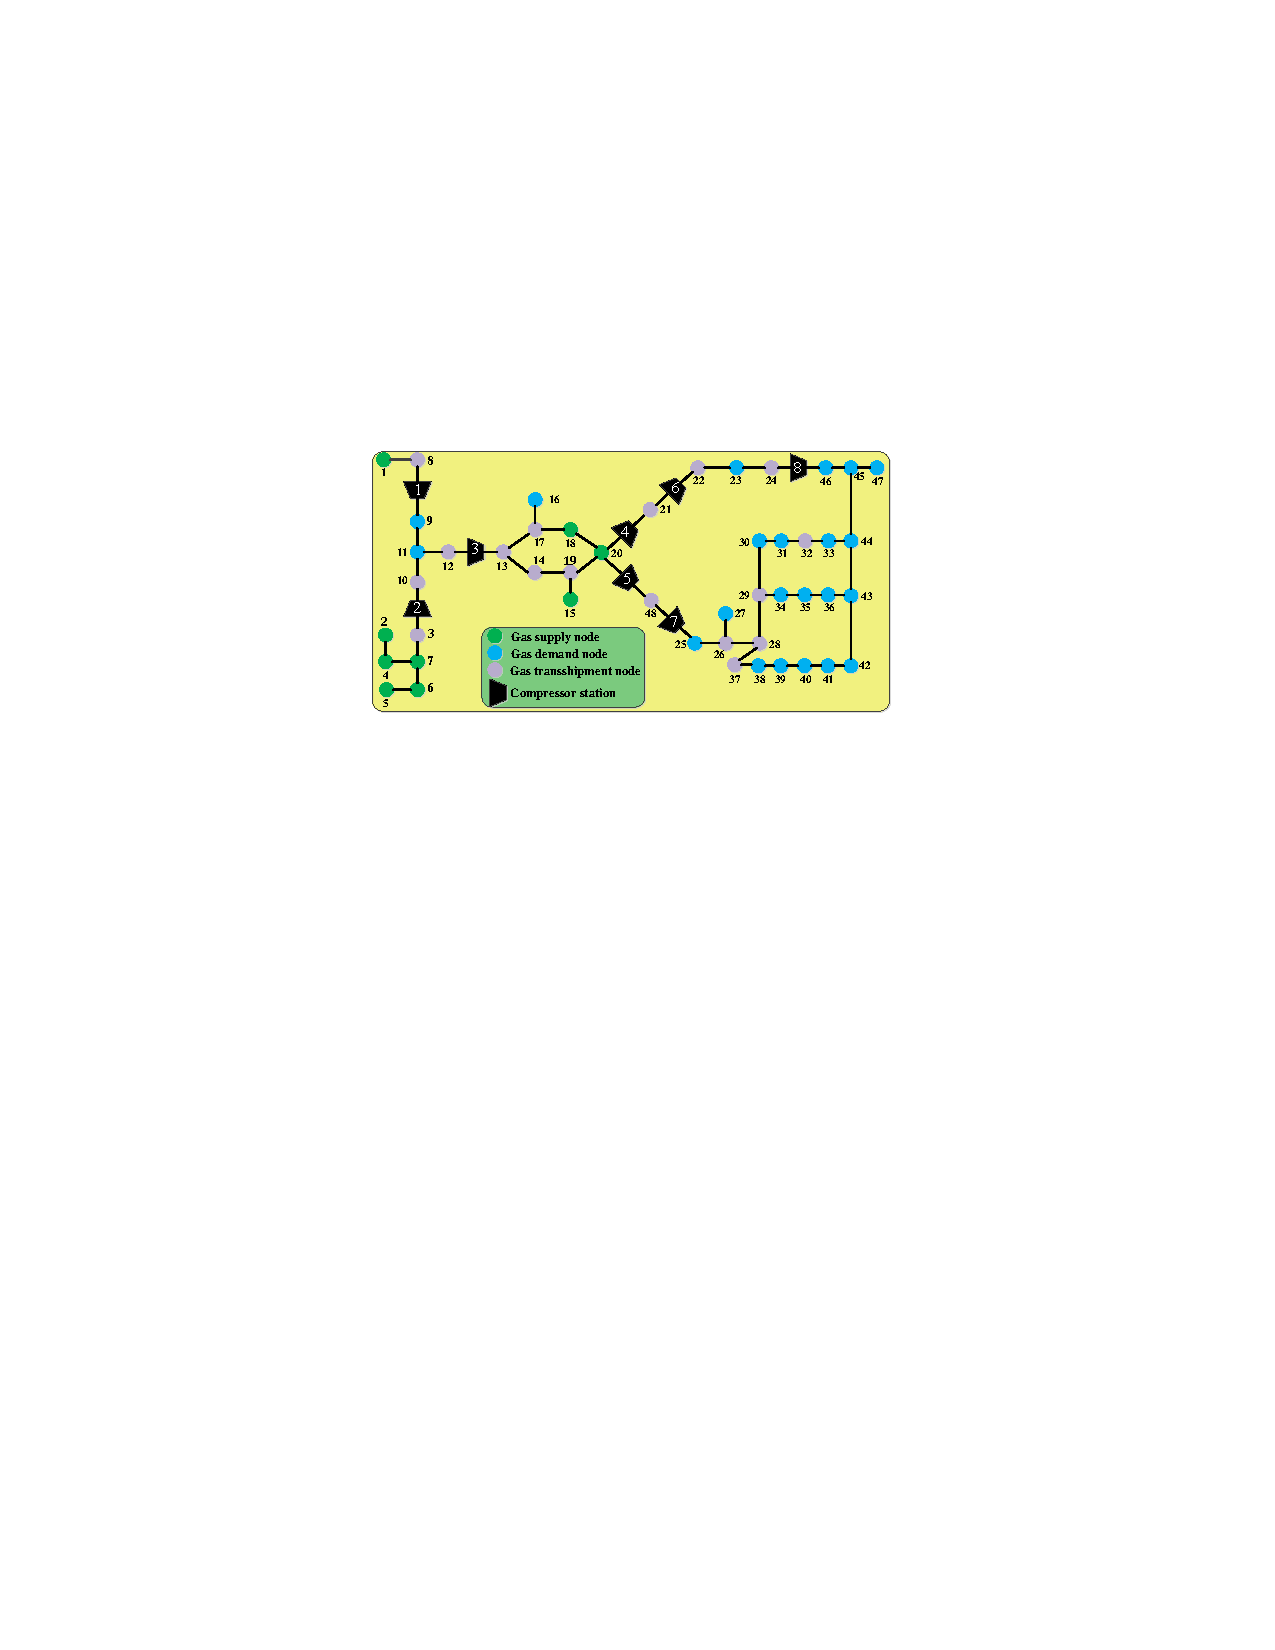
\includegraphics[scale=1.6]{Figures/NG48}
\caption{Natural gas network for Example 2. Source:~\cite{Chen2017}.}
\label{fig:ng48}
\end{figure}

In terms of computational and mathematical tractability, looped natural gas systems are the most complex to solve because they require nodal pressures that guarantee the gas flow in more than one pipeline~\cite{Woldeyohannes2011}. This states an interesting scenario to assess the performance of \mpng{}. In this example, we consider two case studies over the 48-node gas network: a \textit{base case} study, where elements interact properly in a normal operation with no perturbations; and a \textit{contingency case} study, where failures lead to complex decisions for the simulator.

Following Example \ref{sec:8-9_gas_power}, we start by defining all the power, gas, and connect constants. Then, we load the corresponding cases for this example: the gas case (\code{ng\_case48}), and the straightforward 2-bus power system (\code{case2}) that allows the virtual connection to the natural gas system (\code{connect\_pg\_case2}) with minimal implications in topological and computational terms. Lastly, we package the cases and the connect struct together and  run \mpng{}:

\begin{Code}
mpc = loadcase(`case2');        % 2 bus power system 
mgc = ng_case48;                % 48 node looped natural gas system
connect = connect_pg_case2;     % interconnection case

%% put cases together
mpgc = mpc;                     % initialize MPNG case
mpgc.mgc = mgc;                 % adding gas case
mpgc.connect = connect;         % adding connection struct

%% run mpng
res_base = mpng(mpgc,mpopt);         % running MPNG
\end{Code}

Now, we modify the base case to obtain the \textit{contingency case}. Specifically, we reduce the maximum injection capability of one of the wells located at the network center (node 20), forcing the system to extract natural gas from somewhere else to fulfill the gas demand. Moreover, we set pipeline number 38 (the one that connects nodes 43 and 44) to be out of service, eliminating one of the gas network loops located downstream. This contingency forces the system to supply the demands of nodes 30 to 33 through only two paths, which might cause over-pressures and pipeline congestion. 

To simulate these contingencies, we start again by loading the 48-node gas case. Then, we set the reduced maximum injection for well 9. For eliminating the mentioned pipeline, we remove its whole corresponding row in the field \code{mgc.pipe}. Once the contingencies are properly modeled, we put the entire system together and finally rerun the program:

\begin{Code}
%% changes due to contingencies
mgc_cont = mgc;
mgc_cont.well(9,GMAX) = 200;        % set max injection of well 9
cont_pipe = 39; 		    % id for out-of-service pipeline	 
mgc_cont.pipe(cont_pipe,:) = [];    % take pipeline out of service

%% putting all together
mpgc_cont = mpc;                    % initialize MPNG case
mpgc_cont.mgc = mgc_cont;           % adding gas case
mpgc_cont.connect = connect;	% adding connection struct

%% running program 
res_cont = mpng(mpgc_cont,mpopt);   % running MPNG
\end{Code}

Figures \ref{fig:ex2_pressure} to \ref{fig:ex2_inj} show the results comparison between the base case and the contingency case. We mainly analyze pressures, gas flows, and well injections, since they are the most representative variables in the gas network. As seen, reducing the injection capacity in node 22 leads not only to the maximum injection in node one but also to the activation of the wells located at nodes 2 and 6 to balance the global production. As a consequence, new gas flows appear through pipelines 4-7 and 6-7 as a result of higher pressures in nodes 2 to 7; moreover, the gas flow through pipe 1-8 increases at the expense of lower pressure of node 8. Besides, compressors 1, 2, and 3 are forced to transport larger flows by increasing the difference between suction and discharge pressures, that is, their compressor ratios. On the other hand, the outage of pipeline 43-44 leads to higher pressures in the surrounding nodes because of the new radial connections of some pipes. Notice how pipelines 36-43 and 43-42 end up with gas flows in the opposite direction in the contingency case.

\begin{figure}[H]
\centering	
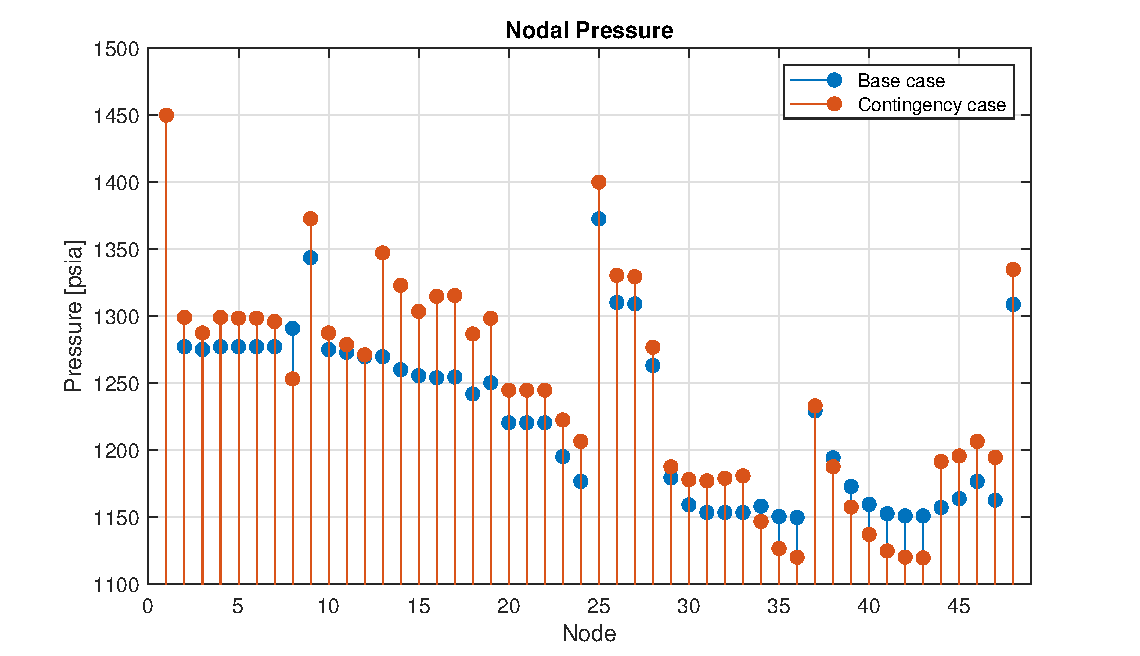
\includegraphics[scale=0.8]{Figures/ex2_pressure}
\caption{Results Example 2 - Nodal Pressure.}
\label{fig:ex2_pressure}
\end{figure}

\begin{figure}[H]
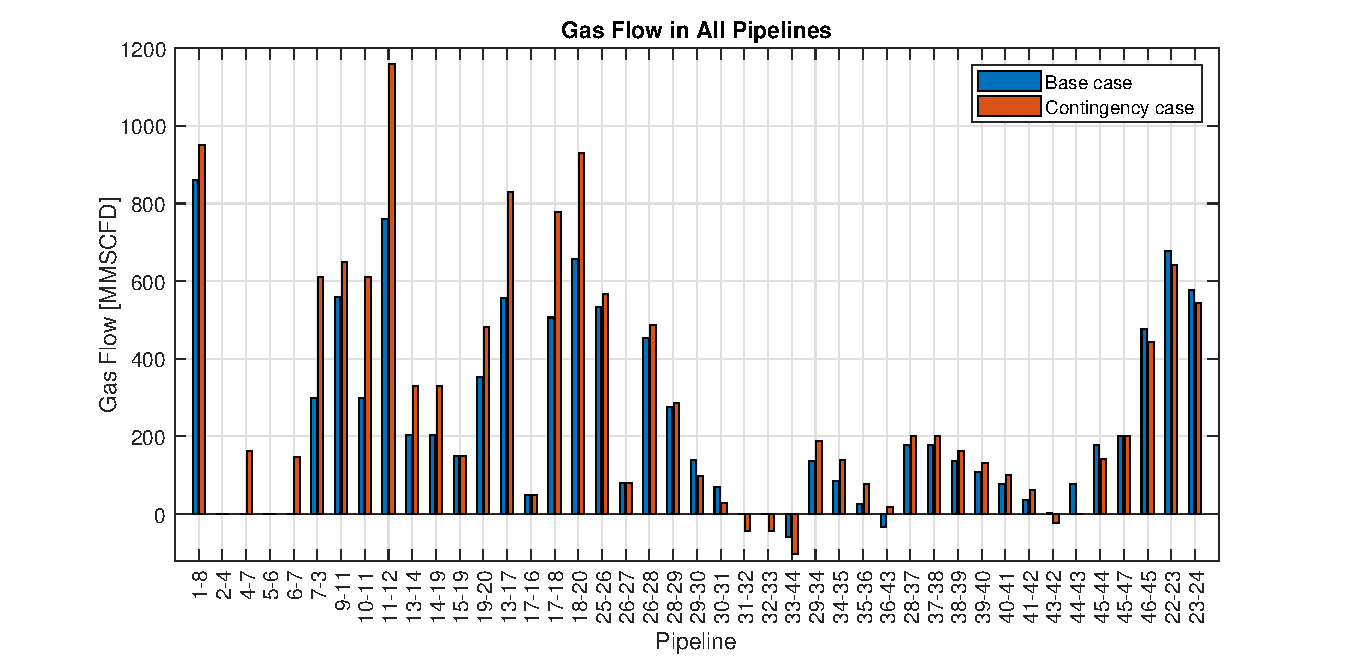
\includegraphics[scale=0.75]{Figures/ex2_fgo}
\caption{Results Example 2 - Gas Flow Through Pipelines.}
\label{fig:ex2_fgo}
\end{figure}

\begin{figure}[H]
\centering
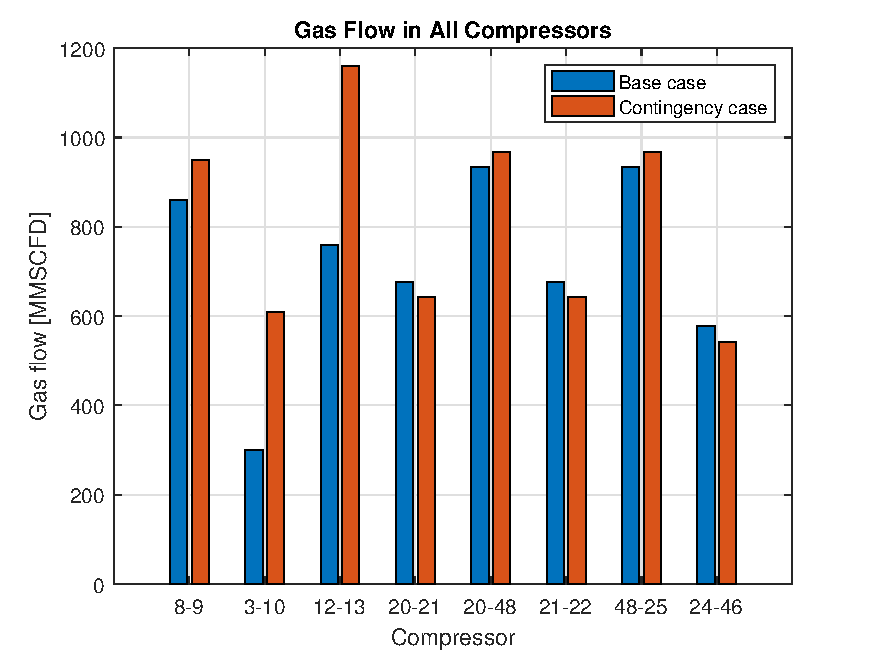
\includegraphics[scale=0.8]{Figures/ex2_fgc}
\caption{Results Example 2 - Gas Flow Through Compressors.}
\label{fig:ex2_fgc}
\end{figure}

\begin{figure}[H]
\centering
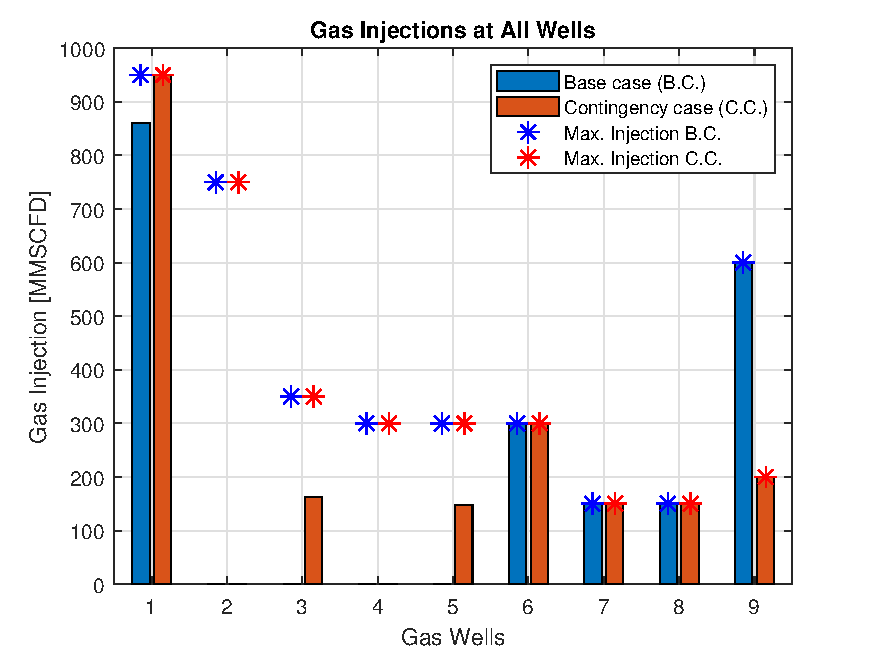
\includegraphics[scale=0.8]{Figures/ex2_inj}
\caption{Results Example 2 - Gas Injection in Wells.}
\label{fig:ex2_inj}
\end{figure}

